\chapter{Syntax}\label{chap:syntax}

To describe the formal syntax of \gls{gamble}, and to parse the language, it is necessary to write a \acrfull{cfg}.
This chapter will explain what a \acrshort{cfg} is, and the problems of creating one.
After this explanation our own \acrshort{cfg}, will be presented.

\section{Context-Free Grammar}\label{sec:cfg}
A \acrshort{cfg} is an area of formal languages which are useful for specifying syntax. 
A \acrshort{cfg} consists of one or several production rules.
On the left side of a production rule is a non-terminal and on the right side are terminals and/or non-terminals, additionally there is a start symbol.
An example of this is written in \myref{lst:cfglst1}, where a definition for multiplication and addition with parenthesis is shown.
The expression production on this figure uses left recursion, since an expression has a production which first element is also an expression.
The grammar is structured such that the multiplication operator have a higher precedence than the addition operator.

\begin{lstlisting}[caption={An example of a \acrshort{cfg} written in \acrshort{ebnf}, with \acrshort{regex} for defining numbers. },frame=tlrb,label={lst:cfglst1},numbers=none]
expression = term | expression "+" term;
term       = factor | term "*" factor;
factor     = constant | "(" expression ")";
constant   = [0-9]+
\end{lstlisting}

It is possible to generate a parse tree for a string which follows the grammar. 
If there exists two or more trees for any given string then the grammar is ambiguous. 
Having an ambiguous grammar can be a problem when parsing because the parser cannot always decide which grammar rule it has to apply.
Ambiguity is a feature of the grammar, not the language. 

\subsection{The dangling else problem}
This section shows an example of how to change grammar's ambiguity problems, some tools can for generating parsers from grammar's, can solve these problems themselves.
One of these tools \acrshort{antlr} will be discussed later in \todo{ref til \acrshort{antlr}}.

A common mistake leading to ambiguous grammar is the dangling else problem. \citep{danglingelse}
In many programming languages it is possible to have an if statement and an else statement, and inside the body of these also having if- and else statements. 
A \acrshort{cfg} describing it is shown in \myref{lst:danglingelseex1}.

\begin{lstlisting}[caption={An example of a \acrshort{cfg} describing an if statement. \citep{danglingelse}},frame=tlrb,label={lst:danglingelseex1},numbers=none]
if statement =
    | if clause statement
    | if clause statement else statement

statement =
    | simple statement
    | if statement
    | loop statement
\end{lstlisting}

Given an input where the statement of an if statement contains another if statement this grammar is ambiguous.  
However it can be rewritten to allow if- and else statements in a grammar, yet this will in almost all cases cause the size of the grammar to increase. 
A solution to this problem is to observe that there exists two kinds of if statements, open and closed if statements.
An open statement is one which the if statement is not paired with an else, and a closed statement is any if statement paired with an else.
A simple statement is also a closed statement.
A simple statement is any regular statement, i.e. Assignment.
A grammar resolving the dangling else problem using this method is shown in \myref{lst:danglingelseex2}.

\begin{lstlisting}[caption={An example of a \acrshort{cfg} describing an if statement, that is not ambiguous. \citep{danglingelse}},frame=tlrb,label={lst:danglingelseex2},numbers=none]
statement =
    | open statement
    | closed statement

open statement =
    | if clause statement
    | if clause closed statement else open statement

closed statement =
    | simple statement
    | if clause closed statement else closed statement
\end{lstlisting}

Another way to resolve this issue is to force statement bodies of if statements, when followed by else statement, to be delimited by explicit blocks, such as \texttt{begin..end} used in Pascal or curly brackets (\texttt{\{...\}}) used in C and derivatives. 

\subsection{Derivations of parse trees}\label{sec:parsetrees}
A parser is a program which takes a string of symbols, and parses it into segments according to the rules specified in a grammar.
A more thorough explanation of parsers can be found in \myref{subsec:parser}
Two common strategies to generate a parse tree is leftmost derivation and rightmost derivation. 
A leftmost derivation applies the rules in the grammar by always applying a production rule to the leftmost non-terminal. 
This is the strategy used in a top-down parser, also known as an LL parser.
A rightmost derivation is the reverse, and what is used in a bottom-up parser, also known as a LR parser. 

%For example take the string: ``1 + 3 * 4'', following PEMDAS this results in 13, if one were to simply calculate from left to right the result would be 16.
%A leftmost derivation would be:
%
%\begin{table}
%    \centering
%    \colorlet{shadecolor}{gray!40}
%    \rowcolors{1}{white}{shadecolor}
%    \begin{tabular}{|l|l|l|}
%    \hline
%    \textbf{Step} & \textbf{Sentential Form}           & \textbf{Production Number} \\ \hline
%    1    & \textit{expression}                &                   \\ \hline
%    2    & \textit{expression} ``+'' \textit{term}       & 1                 \\ \hline
%    3    & \textit{term} ``+'' \textit{term}             & 1                 \\ \hline
%    4    & \textit{factor} ``+'' \textit{term}          & 2                 \\ \hline
%    5    & \textit{constant} ``+'' \textit{term}         & 3                 \\ \hline
%    6    & 1 ``+'' \textit{term}                & 4                 \\ \hline
%    7    & 1 ``+'' \textit{term} ``*'' \textit{factor}     & 2                 \\ \hline
%    8    & 1 ``+'' \textit{constant} ``*'' \textit{factor} & 3                 \\ \hline
%    9    & 1 ``+'' 3 ``*'' \textit{constant}      & 3                 \\ \hline
%    10   & 1 ``+'' 3 ``*'' 4             & 4                 \\ \hline    
%    \end{tabular}
%    \caption{Existing GPU supporting languages}
%    \label{tbl:sota}
%\end{table}

\section{Classes of CFGs}
As mentioned there are two common strategies for parsing, leftmost and rightmost. 
A parser also has a lookahead which is the maximum numbers of tokens which are needed to determine what rule should be applied, this is denoted in a parenthesis, so i.e. LL(1) means leftmost derivation using a lookahead of 1 token. 
A lookahead of k means that there is a constant lookahead of a maximum of k tokens for the given parser. 
There also exists the LL(*) which can dynamically change the number of tokens needed to parse by recognizing if they follow a \acrshort{regex}.
An LL parser is called an LL(*) parser if it is not limited to finite k tokens of lookahead, but can make parsing decisions by recognizing whether the following tokens belong to a regular language.
Combining this with the fact that any LL grammar is a special case of a LR grammar and the different cases of lookahead constructs a hierarchy. 
This hierarchy is shown in \myref{image:hierarchyofgrammars}, LL(*) is not included.
This figure is also contains the Simple LR which is more powerful than a LR(0) grammar, but less than a LR(1), and the LALR(1) which is more powerful than Simple LR and less than LR(1).
More powerful means that a grammar following it can produce more languages typically a superset of another. 
\begin{figure}[!ht]
\centering
 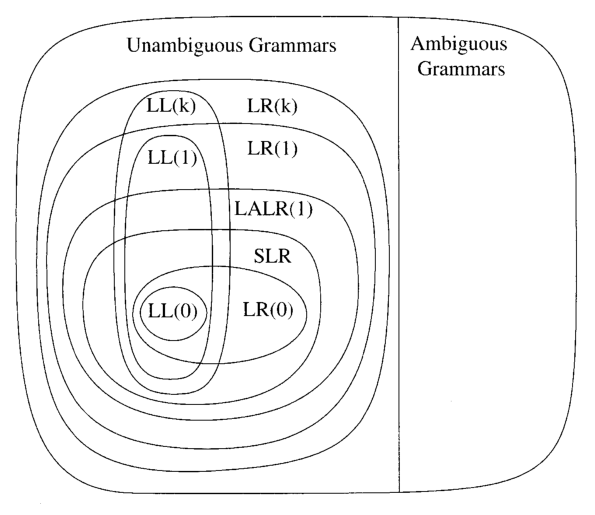
\includegraphics[width=0.5\textwidth]{figures/classesofgrammars.png} % trim=4.85cm 15cm 0.85cm 1cm
\caption{The hierarchy of \acrlong{cfg}. \citep{NvidiaCUDASeminar} \todo[inline]{TODO: Tikz figur med LL(*) indsat.}}\label{image:hierarchyofgrammars}
\vspace{-15pt}
\end{figure}
\section{Context free grammar in GAMBLE}
\gls{gamble}'s grammar is written in \acrfull{ebnf}, and uses regular expressions to define terminals such as numbers and identifiers.
In this section there will be a short traversal of a branch from the parse tree.\todo{Hvad ? hvad betyder det??? - Søren}
The full \acrshort{cfg} of \gls{gamble} can be found in \myref{app:CFG} alongside the lexing rules.
This section only presents a small selection of the \acrshort{cfg}.
\gls{gamble}s \acrshort{cfg} is used in the compiler for parsing a program into a structure, which can be manipulated and analysed to produce the target code for the specific program.\todo{Er det vigtigt ? Kan vi ikke nøjes med at sige at grammatikken skal bruges til en parser for gamble ? Vi forklarede det jo i sidste afsnit ? - Søren}
The production rules are used to check for any syntactical errors which might occur.

A production rule from the \acrshort{cfg} of \gls{gamble} is the statement rule. 
Looking at \myref{lst:statements} it is seen that a statement can be both an assignment, declaration, functioncall, controlblock or a loop construct. 
Statement productions are the building blocks of any source code written in \gls{gamble}.

\begin{lstlisting}[caption={\acrshort{cfg} Statement},frame=tlrb,label={lst:statements},numbers=none]
statement
    : assignment ';'
    | declaration ';'
    | functioncall ';'
    | controlblock 
    | loop
    ;
\end{lstlisting}

All production rules in the statement each expand to their own production hence they are non-terminals.
Looking at the declaration production on \myref{lst:declaration} observe that it has two production rules, \texttt{datatype '=' expression} and \texttt{complexdatatype ID '=' expression}. 
They both end on the expression production which can be seen on \myref{lst:expression}.

\begin{lstlisting}[caption={\acrshort{cfg} Declaration},frame=tlrb,label={lst:declaration},numbers=none]
declaration
    : datatype ID '=' expression                        #primitiveDecl
    | complexdatatype ID '=' expression                 #complexDecl
    ; ;
\end{lstlisting}\todo{Er denne rigtig i forhold til den nye grammatik der er blevet lavet igennem tiden ? Den opdaterede grammatik skal også sættes ind i appendix - Søren}

Further expanding into the expression production rules, it can be seen that it has five different production rules.
An expression has production rules expanding the expression into a construct containing more expressions.
This is done because an expression can derive to a value, and several values are needed for multiple arithmetic operations.
This construct also causes left-recursion, something often attempted to be avoided in \acrshort{cfg}.
The parse generator \acrshort{antlr} can handle simple left-recursion as seen on \myref{lst:value} and as such it is acceptable in the \acrshort{cfg} for \gls{gamble}.\todo{Måske vi skal have et afsnit inden gamble CFG omkring parse generators eller noget ? :) Det skal bare nævnes et sted - Søren}
It does so internally rewriting it and as such removes the left-recursion.
\begin{lstlisting}[caption={\acrshort{cfg} Expression},frame=tlrb,label={lst:expression},numbers=none]
expression
    : expression ( '*' | '/' | '%' ) expression     #mulExpr
    | expression ( '+' | '-' ) expression           #addExpr
    | '(' expression ')'                            #parenExpr
    | value                                         #valueExpr
    | ID postUnaryOperator                          #postIDExpr
    ;
\end{lstlisting}
  
The value production rule can expand into what is seen on \myref{lst:value}.
In this production both terminals and non-terminals are included.
The terminals are elements that have no further production rules, leading to a ``dead end''.
When a terminal is reached it is encountered the deriviation ends and the terminal becomes a leaf on the parse tree, also seen in \myref{sec:AST}.
\begin{lstlisting}[caption={\acrshort{cfg} Value},frame=tlrb,label={lst:value},numbers=none]
value
    : ID                                     #valID
    | constant                               #valConstant
    | '[' valueList ( ';' valueList )* ']'   #valList
    | functioncall                           #valFuncCall
    | collectionEntrance                     #valCollectionEntrance
    | BOOLVAL                                #valBool
    ;
\end{lstlisting}\todo{Er de rent faktisk terminals ? Er en terminal ikke noget som ikke har en productionrule ? Det har de vel allesammen her ?}
\todo[inline]{burde vi ikke beskrive alternative labels aka hashtags #? MP}


